\documentclass{article}
\usepackage{amsmath}
\usepackage{amsthm}
\usepackage{pgfplots}
\usepackage[margin=1in]{geometry}
\usepackage{listings}
\begin{document}
\begin{flushright}MAT 128A: Homework 1\\ Hangshi Jin\\ 913142686\\ Rohit Thomas
\end{flushright}
\begin{large}Section 1.1\end{large}
\\\\10(a)
\[f'(x)=e^x\cos{x}-e^x\sin{x},f''(x)=-2e^x\sin{x},f'''(x)=-2e^x\sin{x}-2e^x\cos{x}\]
\[P_2(x)=f(\frac{\pi}{6})+(e^\frac{\pi}{6}\cos{\frac{\pi}{6}}-e^\frac{\pi}{6}\sin{\frac{\pi}{6}})(x-\frac{\pi}{6})-e^\frac{\pi}{6}\sin{\frac{\pi}{6}}(x-\frac{\pi}{6})^2\]
\[P_2(0.5)=1.44687901012,R_2(0.5)=\frac{f'''(X)}{6}(0.5-\frac{\pi}{6})\]
\[\Rightarrow\text{upper bound for error}=\frac{f'''(\frac{\pi}{6})}{6}(0.5-\frac{\pi}{6})=0.0000101018750376\]
\[\text{actual error}=|P_2(0.5)-f(0.5)|=0.00001002646<\text{upper bound for error}\]
(b)\[R_2(x)=\frac{f'''(X)}{6}(x-\frac{\pi}{6})\]
\[\Rightarrow f'''(1)\leq f'''(X)\leq f'''(0)\Rightarrow |R_2(x)|\leq\frac{2e(\sin{1}+\cos{1})}{6}\left(1-\frac{\pi}{6}\right)^3\]
\[\Rightarrow |P_2(x)-f(x)|\leq0.135371932212\]
(c)\[\int_0^1P_2(x)dx=f(\frac{\pi}{6})+\frac{1}{2}(e^\frac{\pi}{6}\cos{\frac{\pi}{6}}-e^\frac{\pi}{6}\sin{\frac{\pi}{6}})-(e^\frac{\pi}{6}\cos{\frac{\pi}{6}}-e^\frac{\pi}{6}\sin{\frac{\pi}{6}})\frac{\pi}{6}-\frac{1}{3}e^\frac{\pi}{6}\sin{\frac{\pi}{6}}+\frac{\pi}{6}e^\frac{\pi}{6}\sin{\frac{\pi}{6}}-\frac{\pi^2}{36}e^\frac{\pi}{6}\sin{\frac{\pi}{6}}=1.376541852\]
\[\int_0^1f(x)dx=\left. e^x\sin{x}\right|_0^1-\int_0^1e^x\sin{x}dx=\left.\frac{e^x\sin{x}+e^x\cos{x}}{2}\right|_0^1=1.37802461355\]
(d)\[\int_0^1|R_2(x)|dx\leq1\cdot0.135371932212=0.135371932212\]
\[\text{actual error}=|1.376541852-1.37802461355|=0.00148276155\]
\begin{large}Section 1.2\end{large}
\\\\1(a)\[\text{absolute error}=|\pi-\frac{22}{7}|=0.00126448926735,\text{relative error}=\frac{|\pi-\frac{22}{7}|}{\pi}=0.000402499434771\]
2(a)\[3.14127849432=10^{-4}\cdot\pi-\pi\leq\text{approx}\leq10^{-4}\cdot\pi+\pi=3.14190681286\]
6(a)\[\text{absolute error}=|133.921-133.9|=0.021,\text{relative error}=\frac{|133.921-133.9|}{133.921}=0.000156808864928\]
8(a)\[\text{absolute error}=|133.921-133.9|=0.021,\text{relative error}=\frac{|133.921-133.9|}{133.921}=0.000156808864928\]
21(b)\[f(x)=1.01\cdot(4.62)^4-(4.62)^4-3.11\cdot(4.62)^2+12.2\cdot4.62-1.99\approx460-455-66.2+56.4-1.99=-6.79\]
(c)\[f(x)=(((1.01e^x-4.62)e^x-3.11)e^x+12.2)e^x-1.99=(((1.01\cdot4.62-4.62)\cdot4.62-3.11)\cdot4.62+12.2)\cdot4.62-1.99=\]
\[=-1.1\cdot4.62-1.99=-7.07\]
(d)\[\text{absolute error of (b)}=|-7.61+6.79|=0.82\geq\text{absolute error of (c)}=|-7.61+7.07|=0.54\]
\begin{large}Section 3.1\end{large}
\\\\2(b)\[L_1(x)=\frac{x-1.6}{-0.35} \text{at} (1.25,\sqrt[3]{0.25}),L_2(x)=\frac{x-1.25}{0.35} \text{at} (1.6,\sqrt[3]{0.6})\]
\[\Rightarrow P_1(x)=\sqrt[3]{0.25}L_1(x)+\sqrt[3]{0.6}L_2(x)=0.609920401012x-0.132439976318\Rightarrow P_1(1.4)=0.721448585099\]
\[\text{absolute error}=|0.721448585099-\sqrt[3]{0.4}|=0.0153577146291\]
\[L_3(x)=\frac{(x-1.25)(x-1.6)}{(1-1.25)(1-1.6)}\text{at} (1,0) ,\]\[L_4(x)=\frac{(x-1)(x-1.6)}{(1.25-1)(1.25-1.6)}\text{at} (1.25,\sqrt[3]{0.25}),\]\[L_5(x)=\frac{(x-1)(x-1.25)}{(1.6-1)(1.6-1.25)}\text{at} (1.6,\sqrt[3]{0.6})\]
\[\Rightarrow P_2(x)=\sqrt[3]{0.25}L_4(x)+\sqrt[3]{0.6}L_5(x)=\]\[-3.1832028313x^2+9.68204847021x-6.49884563891\Rightarrow P_2(1.4)=0.816944670036\]
\[\text{absolute error}=|0.816944670036-\sqrt[3]{0.4}|=0.0801383703079\]
4(b)\[R_1(x)=\frac{-1}{9(x-1)^{\frac{5}{3}}}(x-1.25)(x-1.6)\leq f''(1.25)(1.425-1.25)(1.425-1.6)=0.0342978508027\]
There is no $R_2(x)$ because $f'''(1.4)$ goes to $\infty$.
\\\\6(b)\[L_1(x)=\frac{x-0.25}{-0.5},L_2(x)=\frac{x+0.25}{0.5}\]
\[P_1(0)=\frac{-0.25\cdot1.33203}{-0.5}+\frac{0.25\cdot0.800781}{0.5}=1.0664055\]
\[L_3(x)=\frac{(x+0.25)(x-0.25)}{(-0.5+0.25)(-0.5-0.25)}\]
\[L_4(x)=\frac{(x+0.5)(x-0.25)}{(-0.25+0.5)(-0.25-0.25)}\]
\[L_5(x)=\frac{(x+0.5)(x+0.25)}{(0.25+0.5)(0.25+0.25)}\]
\[P_2(0)=\frac{-0.0625\cdot1.93750}{0.1875}+\frac{-0.125\cdot1.33203}{-0.125}+\frac{0.125\cdot0.800781}{0.375}=0.953123666667\]
\[P_3(0)=\frac{0.25\cdot(-0.25)(-0.5)\cdot1.93750}{(-0.5+0.25)(-0.5-0.25)(-0.5-0.5)}+\frac{0.5\cdot(-0.25)(-0.5)\cdot1.33203}{(-0.25+0.5)(-0.25-0.25)(-0.25-0.5)}+\]\[\frac{0.25\cdot0.5\cdot(-0.5)\cdot0.800781}{(0.25+0.25)(0.25+0.5)(0.25-0.5)}+\frac{0.25\cdot0.5\cdot(-0.25)\cdot0.687500}{(0.5+0.25)(0.5+0.5)(0.5-0.25)}=0.984374\]
8(b)\[|R_1(x)|=|(6x^2-3x+1)(x-0.25)(x+0.25)|\leq f''(-0.25)(-0.0625)=0.1328125>\text{actual error}= 0.0664055\]
\[|R_2(x)|=|(4x-1)(x+0.25)(x+0.5)(x-0.25)|\leq f'''(-0.5)(-0.033009559128)=0.099028677384>\text{actual error}=0.046876333333\]
\\19
\\\noindent\rule{16cm}{0.4pt}\lstinputlisting[language=Matlab]{lagrange.m}\noindent\rule{16cm}{0.4pt}
\\By inputing the data manually, this code results
\[\text{For sample 1:} P_6(x)=0.00004094575679039009825870024494929*x^6 - 0.003671679400198307761332971417005*x^5\]\[ + 0.12690236338593147225691152352726*x^4 - 2.0946390777258137838733713447235*x^3 \]\[+ 16.142724359576068896160569193419*x^2 - 42.643480886166715043720391313974*x + 6.67
\] 
\begin{center}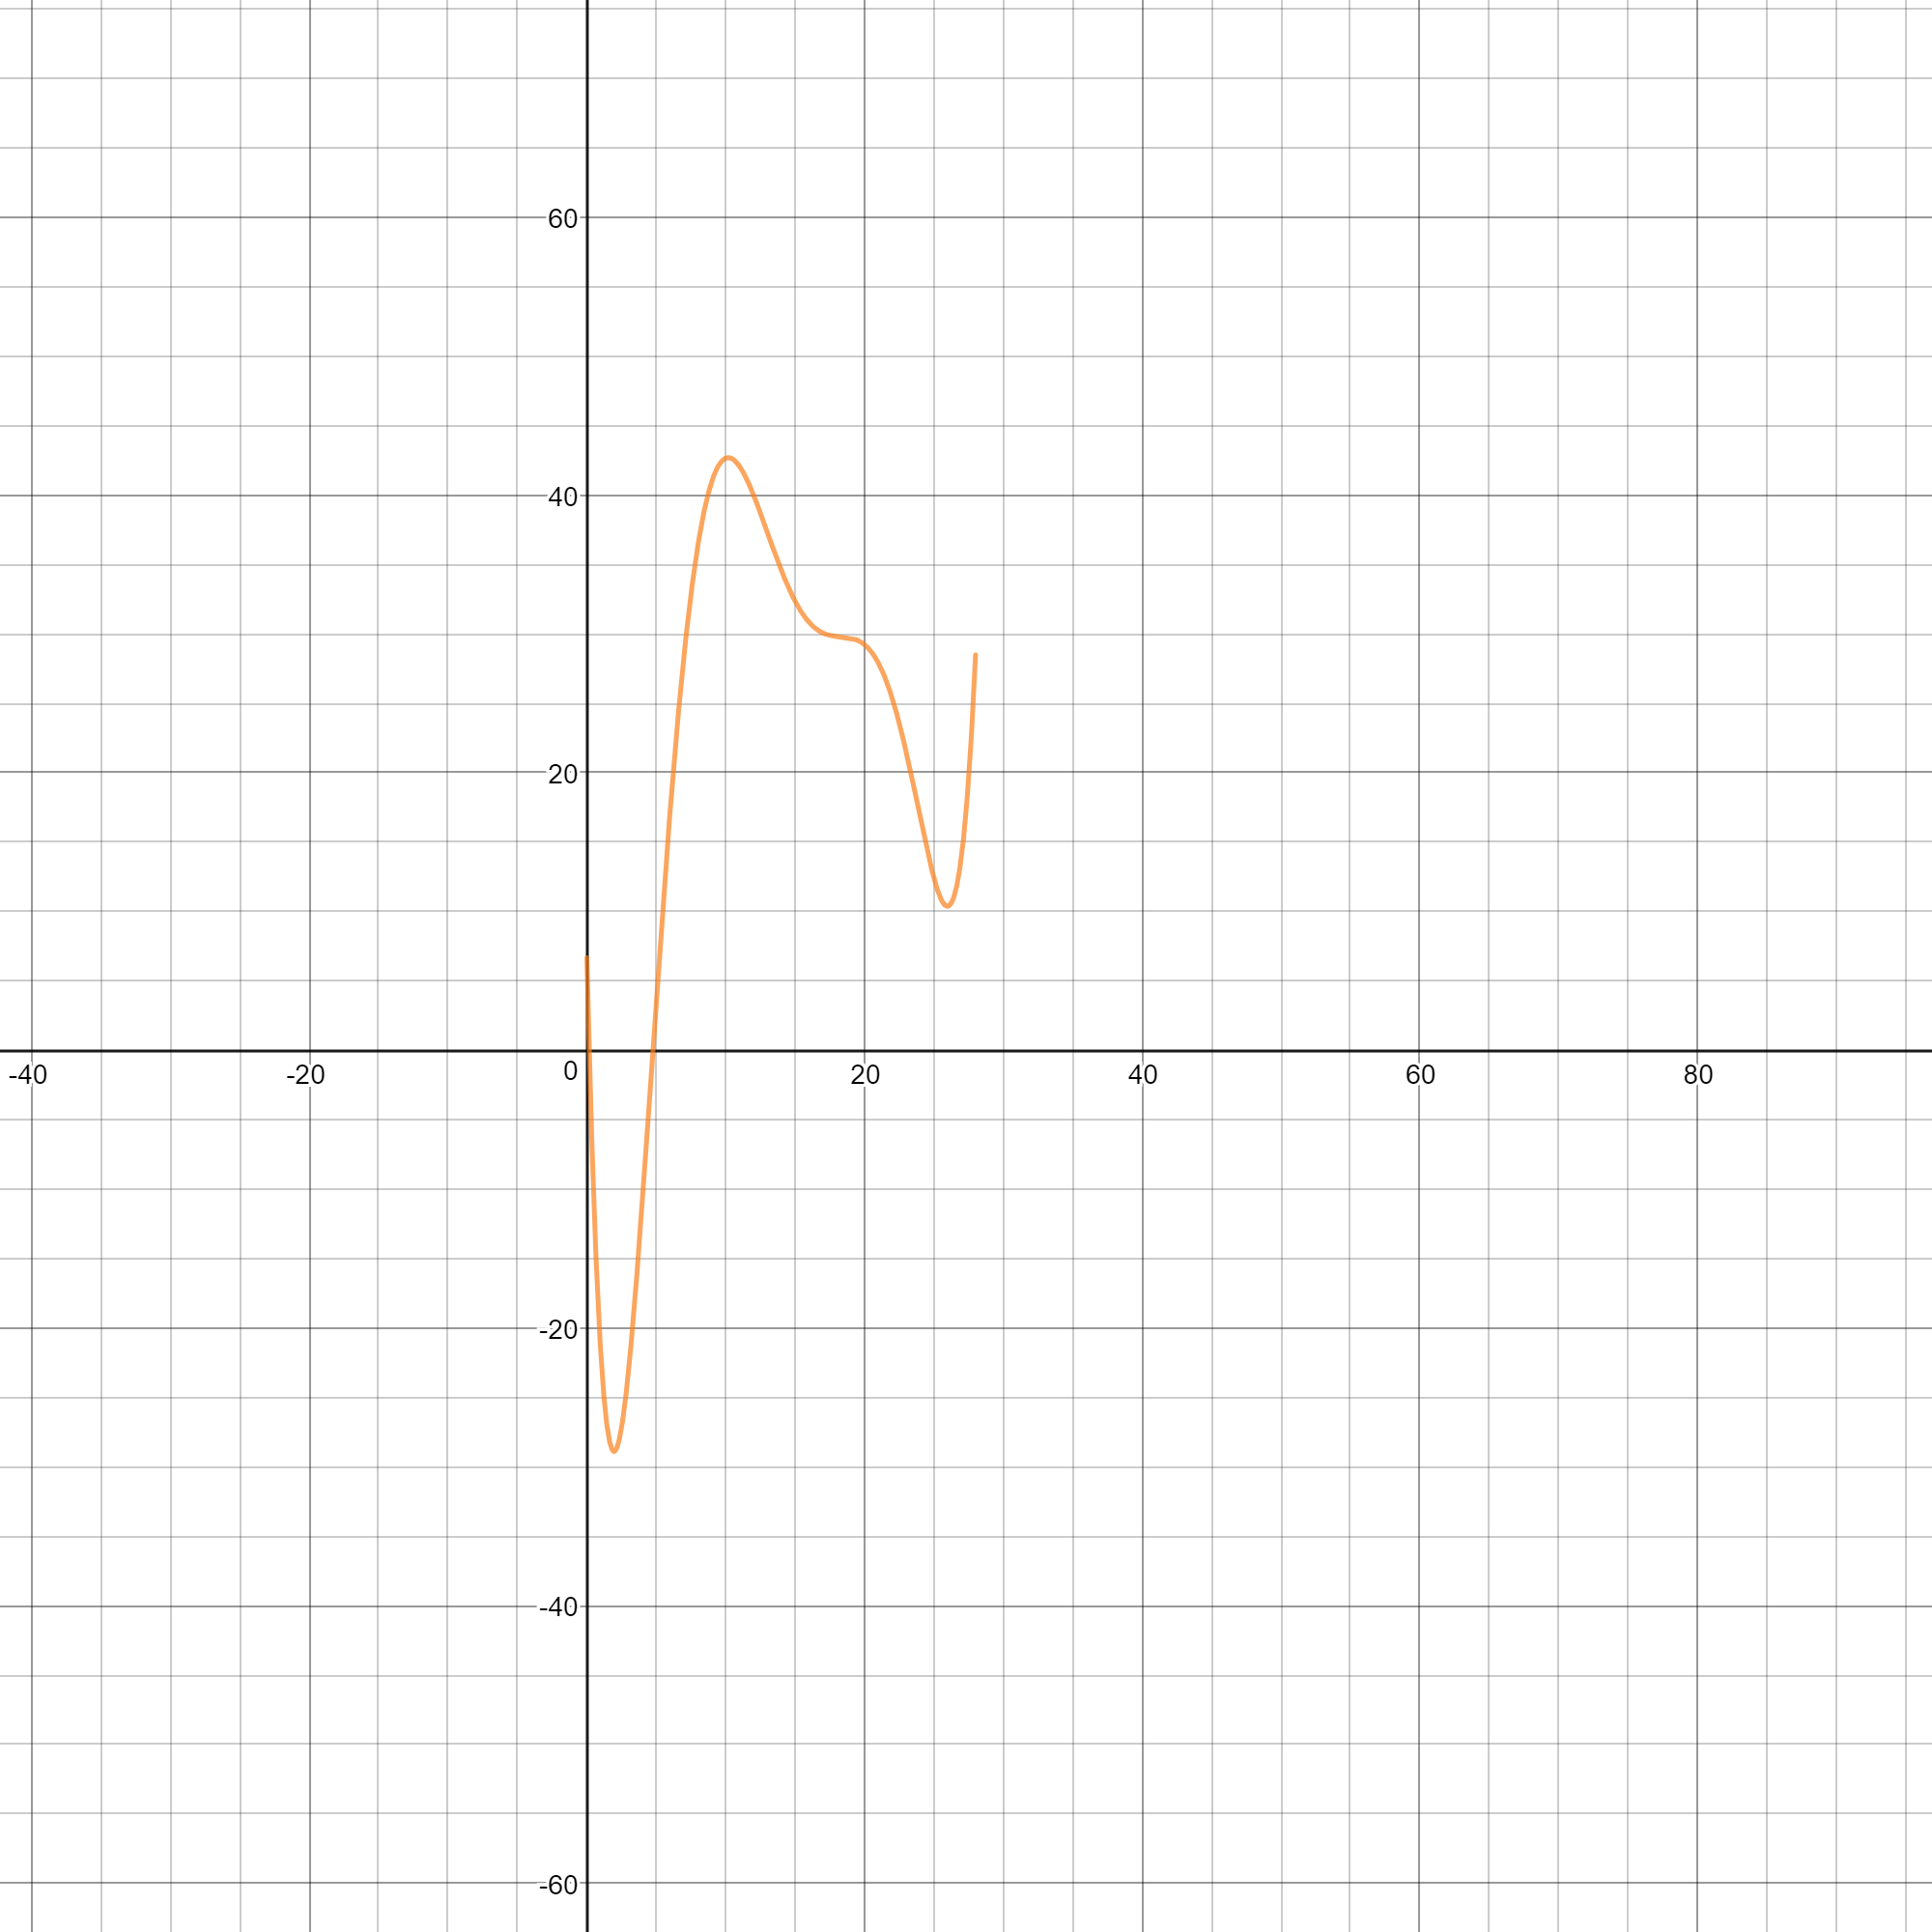
\includegraphics[width=0.5\textwidth]{191}\end{center}\begin{center}Through the graph, we see the approximate maximum average weight for sample 2 is 42.701 mg.\end{center}
\[\text{For sample 2:} P_6(x)=0.0000083615978884313490883391570939317*x^6 - 0.00075254622245168463655858613841807*x^5 \]\[+ 0.025841283442193010565814232735547*x^4 - 0.41379865066497037467243731567643*x^3 \]\[+ 2.9128091017755551750968099325624*x^2 - 5.6782069577778133927866548187404*x + 6.67
\]
\begin{center}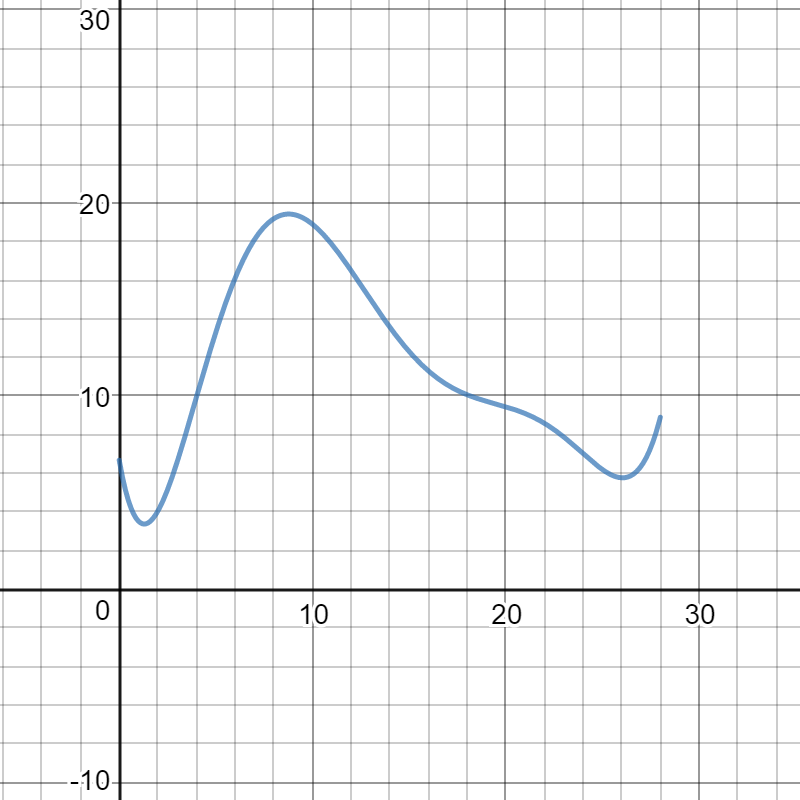
\includegraphics[width=0.5\textwidth]{192}\end{center}\begin{center}Through the graph, we see the approximate maximum average weight for sample 2 is 19.416 mg.\end{center}
\end{document}